\section{Can the VLM drive the design study?}
\label{sec:lo}
\label{sec:qv}
\textbf{Purpose.} This section measures VSPAERO against RANS on the same six geometries and
answers whether the vortex-lattice method can keep driving candidate selection. The comparison
is made at Condition~CR, where both sides share one frame and one geometry set, and it asks two
things: does the low-order method put the candidates in the order the RANS puts them, and how
far off is it on the size of the effect.

\subsection{Method}
\label{sec:qv:vlmmethod}
\textbf{Method.} VSPAERO is a vortex-lattice solver, and it ran the same six geometries that were
meshed. Each deck is matched to its RANS case by \texttt{.vsp3} SHA-256, never by name. All nine
Condition CR decks read $S_\mathrm{ref} = 13.3572$~ft$^2$, so the conversion onto the DSO basis is
exactly 1.000000. The package also carries a second baseline deck, \texttt{baseline\_corrected},
which the design study ranks against; every VLM increment in this report is against the deck of
the meshed baseline B, and referencing it to the other deck moves all five candidates by one
constant and changes no ordering.

\textbf{Which columns compare.} VSPAERO writes $C_{Dtot} = C_{Do} + C_{Di}$, and the decks close
that identity to $10^{-12}$. $C_{Do}$ is a flat-plate skin-friction estimate, and it supplies
40.1 to 41.1~per~cent of $C_{Dtot}$ on the six meshed geometries. The decks evaluate it at
$Re = 1\times10^{7}$, against $Re_{C_\mathrm{ref}} = 0.92\times10^{6}$ here on the same chord. The
defensible drag comparison is therefore induced against induced, and $C_{Dtot}$ appears nowhere
beside a RANS $C_D$. Each VLM induced increment below sits beside the RANS total increment at the
same fixed $C_L$; the RANS induced drag from the Trefftz planes is in Section~\ref{sec:cr:spaneff},
and its span efficiency enters Table~\ref{tab:lo:selection} beside the VLM's own.

\textbf{Result.} Table~\ref{tab:qv:vlm} gives the VLM side, and Figure~\ref{fig:qv:decomp}(a)
draws its composition against the RANS total. The two induced columns differ from each other more
than either differs from anything else. Near-field span efficiency runs $E = 0.57$ to $0.59$,
far-field $E_w = 0.94$ to $0.97$, on the same runs. An independent lifting-line calculation on the
spanwise loading returns 56.9~ct, which supports the far-field column to 0.4~per~cent. Both
columns are carried through the table that follows.
\begin{table}[htbp]
  \centering
  \footnotesize
  \caption{VSPAERO at Condition CR, $M = 0.10$, each deck trimmed to $C_L = 0.428277635108$.
  Drag in counts on the DSO basis, deck $S_\mathrm{ref} = 13.3572$~ft$^2$, conversion onto the
  report basis exactly 1.000000. $C_{Di}$ is the near-field surface integration and $C_{Diw}$ the
  far-field wake integral; $E$ and $E_w$ are their span efficiencies. B is the surface the RANS
  meshes. Source: \texttt{data/vlm.json}.}
  \label{tab:qv:vlm}
  \begin{tabular}{llrrrrrrr}
    \toprule
    Geom. & Deck & $\alpha$ [deg] & $C_{Do}$ & $C_{Di}$ & $C_{Dtot}$ & $C_{Diw}$ & $E$ & $E_w$ \\
    \midrule
    B & \texttt{baseline\_wing\_only\_refined} & 1.99981 & 64.060 & 91.676 & 155.736 & 57.649 & 0.5907 & 0.9394 \\
    C & \texttt{cte\_i002\_c04}                & 1.25652 & 64.078 & 92.342 & 156.421 & 56.258 & 0.5865 & 0.9627 \\
    M & \texttt{mcv2\_i002\_c01}               & 1.24972 & 64.084 & 92.617 & 156.701 & 56.441 & 0.5847 & 0.9595 \\
    F & \texttt{cfft\_b02\_c01}                & 1.45936 & 63.894 & 94.465 & 158.359 & 55.712 & 0.5733 & 0.9721 \\
    W & \texttt{cffw\_b01\_c01}                & 1.42193 & 63.927 & 95.030 & 158.957 & 55.827 & 0.5699 & 0.9701 \\
    H & \texttt{chc\_g02\_c06}                 & 1.44697 & 63.887 & 95.370 & 159.257 & 56.383 & 0.5679 & 0.9605 \\
    \bottomrule
  \end{tabular}
\end{table}

\begin{figure}[htbp]
  \centering
  \begin{subfigure}[t]{0.40\textwidth}
    \centering
    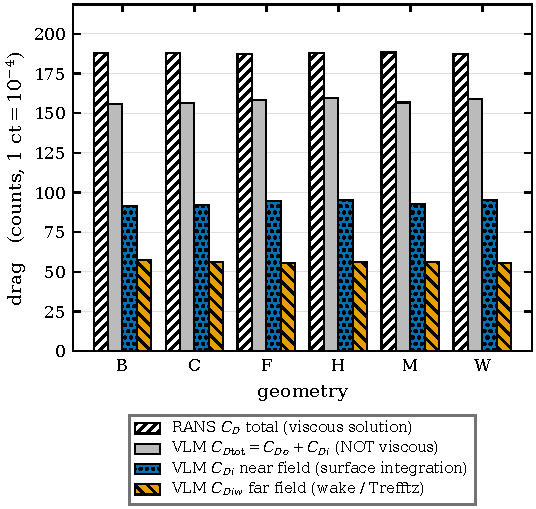
\includegraphics[width=\textwidth]{fig/drag_decomposition_rans_vs_vlm_condition_CR.pdf}
    \caption{Drag decomposition.}
    \label{fig:qv:drag}
  \end{subfigure}
  \hfill
  \begin{subfigure}[t]{0.40\textwidth}
    \centering
    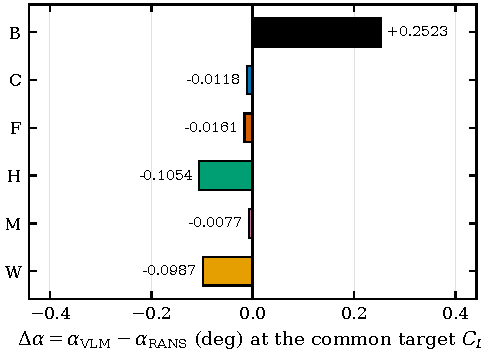
\includegraphics[width=\textwidth]{fig/trim_alpha_rans_vs_vlm_condition_CR.pdf}
    \caption{Trim angle.}
    \label{fig:qv:trimalpha}
  \end{subfigure}
  \caption{Condition CR, $M = 0.10$, $C_L = 0.428277635108$, DSO basis, RANS half model
  $A_\mathrm{ref} = 0.620462$~m$^2$. (a) What each method contains: the RANS total beside the
  VSPAERO $C_{Dtot} = C_{Do} + C_{Di}$ split into its parasite correlation and its induced part,
  with the far-field $C_{Diw}$ alongside. The two bar heights are not differenced, because
  $C_{Do}$ is a flat-plate correlation at the deck Reynolds number. (b) Trim angle at the common
  target $C_L$, which is the closest agreement in this section.}
  \label{fig:qv:decomp}
\end{figure}

\subsection{Drag increments}
\label{sec:qv:counts}
\textbf{Result.} Table~\ref{tab:lo:selection} is the central comparison of this section. The
RANS morphing signal spans $-0.868$ to $+0.232$~ct, $1.100$ in total, and neither VLM column
resolves an effect that small. The near-field column misses the measured increment by $0.709$ to
$4.222$~counts and gets the sign wrong on all four candidates the RANS puts below the baseline.
The far-field column misses by $0.955$ to $1.441$~counts, every error of the same sign and within
half a count of the others, which is why its ordering survives where the near-field ordering does
not: a near-constant offset moves the whole field together and leaves the sequence intact.

\textbf{Far field.} On the far-field column every predicted increment is negative. The VLM has all
five candidates saving induced drag, while the RANS measures four of the five costing total drag.
Those errors run 1.24 to 7.85~ct, and for F, W and H they exceed the entire signal span. Part of
that gap is a real profile increment the VLM has no mechanism to produce, and a RANS Trefftz
integral is what separates the two.

\textbf{Systematics.} The RANS-side systematic uncertainty is far smaller than any of these
differences. Window drift is
0.0014 to 0.0028~ct against a gate of 0.05~ct, and removing each trim case's own $C_L$ residual
moves the increments by at most 0.021~ct.

\begin{table}[htbp]
  \centering
  \scriptsize
  \setlength{\tabcolsep}{3.5pt}
  \caption{Selection test at Condition CR, $M = 0.10$, $C_L = 0.428277635108$, DSO basis (RANS
  half model $A_\mathrm{ref} = 0.620462$~m$^2$; VSPAERO $S_\mathrm{ref} = 13.3572$~ft$^2$,
  conversion exactly 1.000000). Increments are against the baseline B, in counts: the RANS
  increment is a total drag increment and the VLM increments are induced drag increments, so
  ``error'' is the VLM prediction minus the RANS measurement. Ranks are by increasing increment
  against each method's own baseline, rank 1 best; the closest adjacent RANS pair is W and F at $0.053$~ct, so no pair is tied. The last
  three columns are span efficiencies: the VLM's own near- and far-field values, and the RANS
  value at the last Trefftz station. Rows and statistics generated by
  \texttt{scripts/make\_rank\_table.py} from \texttt{fig/fig\_vlmerr\_values.json},
  \texttt{data/vlm.json} and \texttt{data/span\_efficiency.json}.}
  \label{tab:lo:selection}
  \begin{tabular}{lrrrrrrrrrrr}
    \toprule
     & \multicolumn{2}{c}{RANS} & \multicolumn{3}{c}{VLM near field} &
       \multicolumn{3}{c}{VLM far field} & \multicolumn{3}{c}{span efficiency} \\
    \cmidrule(lr){2-3}\cmidrule(lr){4-6}\cmidrule(lr){7-9}\cmidrule(lr){10-12}
    Geom. & $\Delta C_D$ & rank & $\Delta C_{Di}$ & rank & error & $\Delta C_{Diw}$ & rank & error &
      VLM $E$ & VLM $E_w$ & RANS $e$ \\
    \midrule
    W & $-0.868$ & 1 & $+3.354$ & 4 & $+4.222$ & $-1.823$ & 2 & $-0.955$ & 0.5699 & 0.9701 & 0.9837 \\
    F & $-0.815$ & 2 & $+2.789$ & 3 & $+3.604$ & $-1.938$ & 1 & $-1.123$ & 0.5733 & 0.9721 & 0.9859 \\
    C & $-0.191$ & 3 & $+0.666$ & 1 & $+0.857$ & $-1.392$ & 3 & $-1.201$ & 0.5865 & 0.9627 & 0.9773 \\
    H & $-0.009$ & 4 & $+3.694$ & 5 & $+3.703$ & $-1.266$ & 4 & $-1.257$ & 0.5679 & 0.9605 & 0.9773 \\
    M & $+0.232$ & 5 & $+0.941$ & 2 & $+0.709$ & $-1.209$ & 5 & $-1.441$ & 0.5847 & 0.9595 & 0.9724 \\
    \midrule
    \multicolumn{3}{l}{Kendall $\tau$, all five}  & \multicolumn{3}{c}{$-0.20$} & \multicolumn{3}{c}{$+0.80$} & & & \\
    \multicolumn{3}{l}{Spearman $\rho$, all five} & \multicolumn{3}{c}{$-0.20$} & \multicolumn{3}{c}{$+0.90$} & & & \\
    \multicolumn{3}{l}{Pairs swapped, of 10}      & \multicolumn{3}{c}{6} & \multicolumn{3}{c}{1} & & & \\
    \bottomrule
  \end{tabular}
\end{table}

\subsection{Is the ranking preserved?}
\label{sec:qv:rank}
\label{sec:lo:rank}
\label{sec:project:ranking}
\textbf{Result.} Ranking is the property a search tool needs, and it survives on one column
(Table~\ref{tab:lo:selection}), but not the column the June selection was made on. The RANS orders the
candidates $W < F < C < H < M$. Far-field $C_{Diw}$ gives $F < W < C < H < M$, nine of ten pairs
concordant, Kendall $\tau = +0.80$. Near-field $C_{Di}$ gives $C < M < F < W < H$, four of ten
concordant, $\tau = -0.20$.

\textbf{Which way the two metrics fail.} The far-field metric's single error is on the closest
pair in the field: the RANS separates W and F by $0.053$~counts, the narrowest adjacent gap of the
five, and against a convergence gate of $0.05$~counts per window that pair is at the edge of what
this campaign can resolve. A metric that orders everything except the one pair nobody can
separate is performing about as well as the data permits. The near-field metric fails differently
and not by a small margin: $\tau = -0.20$ is worse than no information, because it groups
$\{C, M\}$ as the cheap pair and $\{F, W, H\}$ as the expensive one, and the viscous answer is
close to the reverse.

\textbf{What this claim is not.} The Condition~CR field spans $1.100$~counts and the convergence
gate is $0.05$~counts per window, so the spread is twenty-two gates wide but the closest adjacent
pair is one. Reproducing this ordering is therefore evidence that a metric tracks the sign and the
grouping of the field, not that it resolves neighbours within it; Section~\ref{sec:perf:cr}
makes the same point from the other side, that the low-speed sequence is read as a group. The two
statements are consistent and the distinction is the whole of it: a search tool that puts the
cheap candidates in the cheap group is useful even where it cannot separate two of them, and that
is what $\tau = +0.80$ with its one error on the narrowest pair describes.
\textbf{Reading.} The two induced-drag columns the VLM writes are not interchangeable, and this
is where the choice between them shows. The far-field wake integral is the one that tracks the
viscous ordering; the near-field surface integration does not.

\begin{figure}[htbp]
  \centering
  \includegraphics[width=0.74\linewidth]{fig_vlmerr_ranking.pdf}
  \caption{Selection test at Condition CR, $M=0.10$, every geometry trimmed to
  $C_L = 0.428277635108$ on the DSO basis. Each panel ranks the five candidates by drag
  increment, low order on the left and RANS on the right, rank 1 being the least drag. Panel (a)
  uses near-field $C_{Di}$, the metric the June selection was made on, and swaps 6 of 10 pairs.
  Panel (b) uses far-field $C_{Diw}$, the metric the design study now selects on, and swaps 1 of
  10, that pair being W against F at $0.053$~counts apart. Generated by
  \texttt{fig/make\_vlmerr.py} from \texttt{data/vlm.json} and the Condition CR RANS trims.}
  \label{fig:project-ranking}
\end{figure}

\subsection{Decision}
\label{sec:qv:decision}
\textbf{Decision.} The VLM can be trusted to order candidates, on its far-field column only, and
to price none of them. Ordering: far-field $C_{Diw}$ reproduces the RANS order to nine pairs of
ten, near-field $C_{Di}$ to four of ten. Pricing: the whole morphing effect at Condition CR spans
$1.100$~counts, from W at $-0.868$ to M at $+0.232$, and the far-field increments miss the
measured ones by $0.955$ to $1.441$~counts, which is $87$ to $131$~per~cent of that span. The
near-field increments miss by $0.709$ to $4.222$~counts, $64$ to $384$~per~cent.

\textbf{Why one of them still ranks.} The five far-field errors are all of one sign and lie
within half a count of each other, $-0.955$ to $-1.449$. An error that is nearly a constant offset
moves every candidate together and therefore leaves the ordering intact while destroying the
magnitude, which is precisely the behaviour seen. The near-field errors are neither
one-signed in magnitude nor clustered, spanning a factor of six, and the ordering does not
survive them.

\textbf{Consequence.} Candidate search can stay with VSPAERO provided it selects on the
far-field column, which is the column the design study adopted in its August correction and not
the one the June selection was made on. Every count quoted for a selected concept comes from
RANS, and at Condition CR that is not a refinement but a requirement: the low-order error is the
size of the entire effect being resolved.

\textbf{Consequence for selection.} Both metrics predict a saving for every candidate at
Condition~CR and the viscous calculation returns a saving for four of the five. At cruise it
returns a saving for W alone and a cost for the other four (Section~\ref{sec:cruise}). \textbf{The
three geometries the low-order study currently selects, W, F and H, are the three cheapest at both
cruise points, in that order}. C and M, from the July selection on the near-field column, cost
twelve to fifteen counts.
The cruise cost of C and M is wave drag and separation behind a strong aft shock
(Section~\ref{sec:perf:mechanism}), which no induced-drag column can see, so the selection is
right at cruise for a reason the low-order method does not model. Reselection that admits
strong-camber shapes should therefore rank on a metric that sees the shock; of the two low-order
induced-drag columns, the far-field one is the only one that orders the candidates at low speed.
